\documentclass{article}

\usepackage[english]{babel}
\usepackage[utf8]{inputenc}
\usepackage{amsmath,amssymb}
\usepackage{parskip}
\usepackage{graphicx}
\usepackage{listings}
\usepackage{float}
\usepackage{subfig}
\lstset{
    numbers=left, 
    numberstyle= \tiny, 
    keywordstyle= \color{ blue!70},
    commentstyle= \color{red!50!green!50!blue!50}, 
    frame=shadowbox, % 阴影效果
    rulesepcolor= \color{ red!20!green!20!blue!20} ,
    escapeinside=``, % 英文分号中可写入中文
    xleftmargin=2em,xrightmargin=2em, aboveskip=1em,
    framexleftmargin=2em,
    breaklines=true,
    language=python,
    language=c++,
} 
% Margins
\usepackage[top=2.5cm, left=3cm, right=3cm, bottom=4.0cm]{geometry}
% Colour table cells
\usepackage[table]{xcolor}

% Get larger line spacing in table
\newcommand{\tablespace}{\\[1.25mm]}
\newcommand\Tstrut{\rule{0pt}{2.6ex}}         % = `top' strut
\newcommand\tstrut{\rule{0pt}{2.0ex}}         % = `top' strut
\newcommand\Bstrut{\rule[-0.9ex]{0pt}{0pt}}   % = `bottom' strut

%%%%%%%%%%%%%%%%%
%     Title     %
%%%%%%%%%%%%%%%%%
\title{CSCI803 Assignment}
\author{Yao Xiao \\ SID 2019180015}
\date{\today}

\begin{document}
\maketitle

%%%%%%%%%%%%%%%%%
%   Problem 1   %
%%%%%%%%%%%%%%%%%
\section{Idea}
In fact, the core understanding of the algorithm is to check whether there is a character that satisfies the longest substring condition: the string is displayed as a prefix, suffix, and middle position. He puts the first letter of all strings in the same position at the beginning, because only these positions may have to satisfy the substring condition. Then from front to back, starting from the position, the string that meets condition 1 appears in the middle of the prefix.

In fact, this issue is related to the KMP algorithm. $nxt[i]$ represents the maximum length of the prefix and suffix of the i-th position (after jumping to this position) before and after the i-th position of the same pattern string. Then we can find the next one after the longest common suffix appears in the middle and can be judged, instead of looking at whether there is a secondary suffix in the middle long ago and did the same thing, until we jump to the external string.

So how to determine whether there has been in the middle? We only need to label $nxt[i]$ with the array value that appears on the determined nxt table. Finally, starting from the end position, check whether $nxt[i]$ has marked the value or not, the same suffix length as the middle of the front will be described, not marked in the nxt [$nxt[i]$] double length position, the center mark is not until The mark is found, the record length is exited or the end is not satisfied.


\section{Implementation}
\begin{lstlisting}
#include <iostream>
#include <string>
#define N 1000002
using namespace std;

string s;
int len;
int nxt[N];
int cnt[N];
int length = 0;
int get_next()
{
    int j = 0;
    int k = -1;
    nxt[0] = -1;
    while(j<len)
    {
        if(k==-1||s[k]==s[j])
        {
            ++k;
            ++j;
            nxt[j] = k;
        }
        else
        {
            k=nxt[k];
        }
    }
    for(int i = 0;i<len;i++)
    {
        cnt[nxt[i]] = 1;
    }
}


int main()
{
    cin >> s;
    len = s.size();
    get_next();
    int k = nxt[len];
    int flag = 0;
    while(k>0)
    {
        if(cnt[k])
        {
            flag = 1;
            length = k;
            break;
        }
        k = nxt[k];
    }
    if(flag)
    {
        for(int i = len-length;i<len;i++)
        {
            cout << s[i];
        }
        cout << endl;
    }
    else
    {
        cout << "Just a legend" << endl;
    }
    return 0;
}
\end{lstlisting}

\begin{figure}[H]
    \subfloat{
        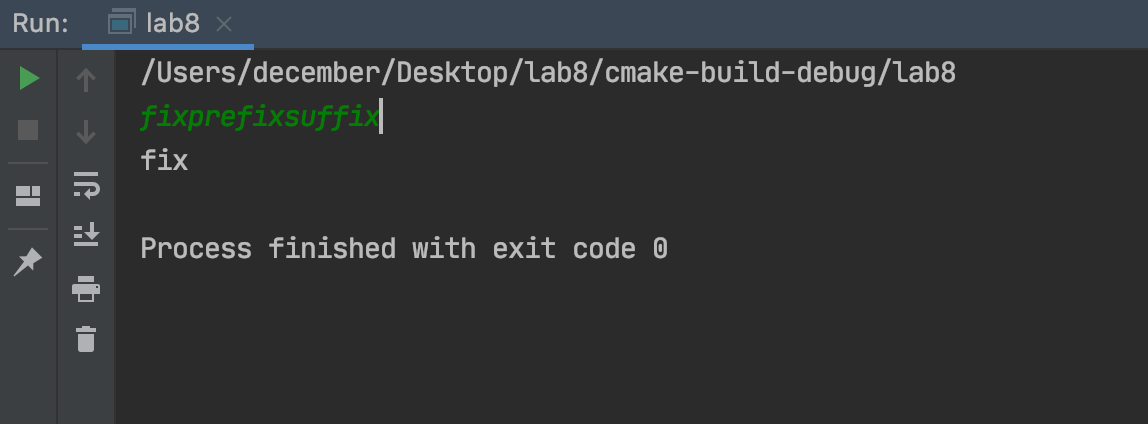
\includegraphics[width=1\textwidth]{Fig1}
    }\\
    \subfloat{
        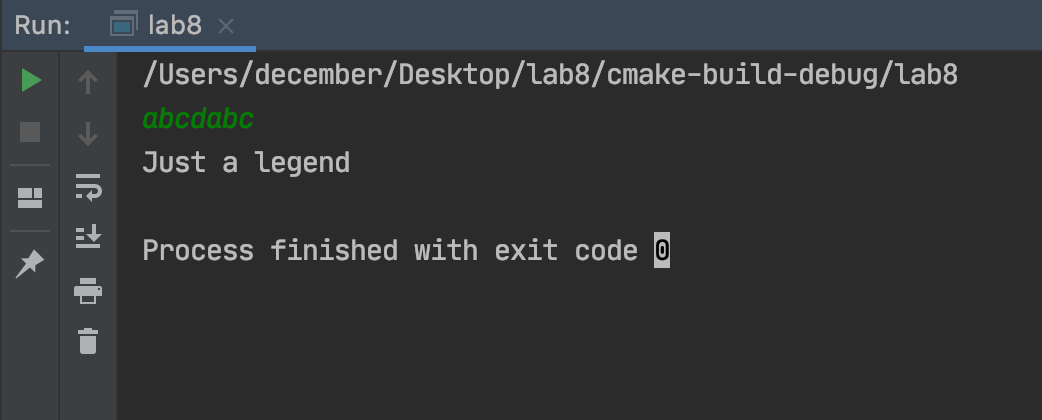
\includegraphics[width=1\textwidth]{Fig2}
    }
\end{figure}
\end{document}
